
\textbf{Descarga de la Imagen de Instalación}
\medskip

Primero, descargamos la imagen de Debian adecuada para nuestras necesidades. Para ello, visitamos la página oficial de Debian en \url{https://www.debian.org/distrib/} y seleccionamos la imagen de instalación que mejor se adapte a nuestro caso. En este ejemplo, se eligió la imagen de instalación a través de Internet.

\begin{figure}[H]
    \centering
    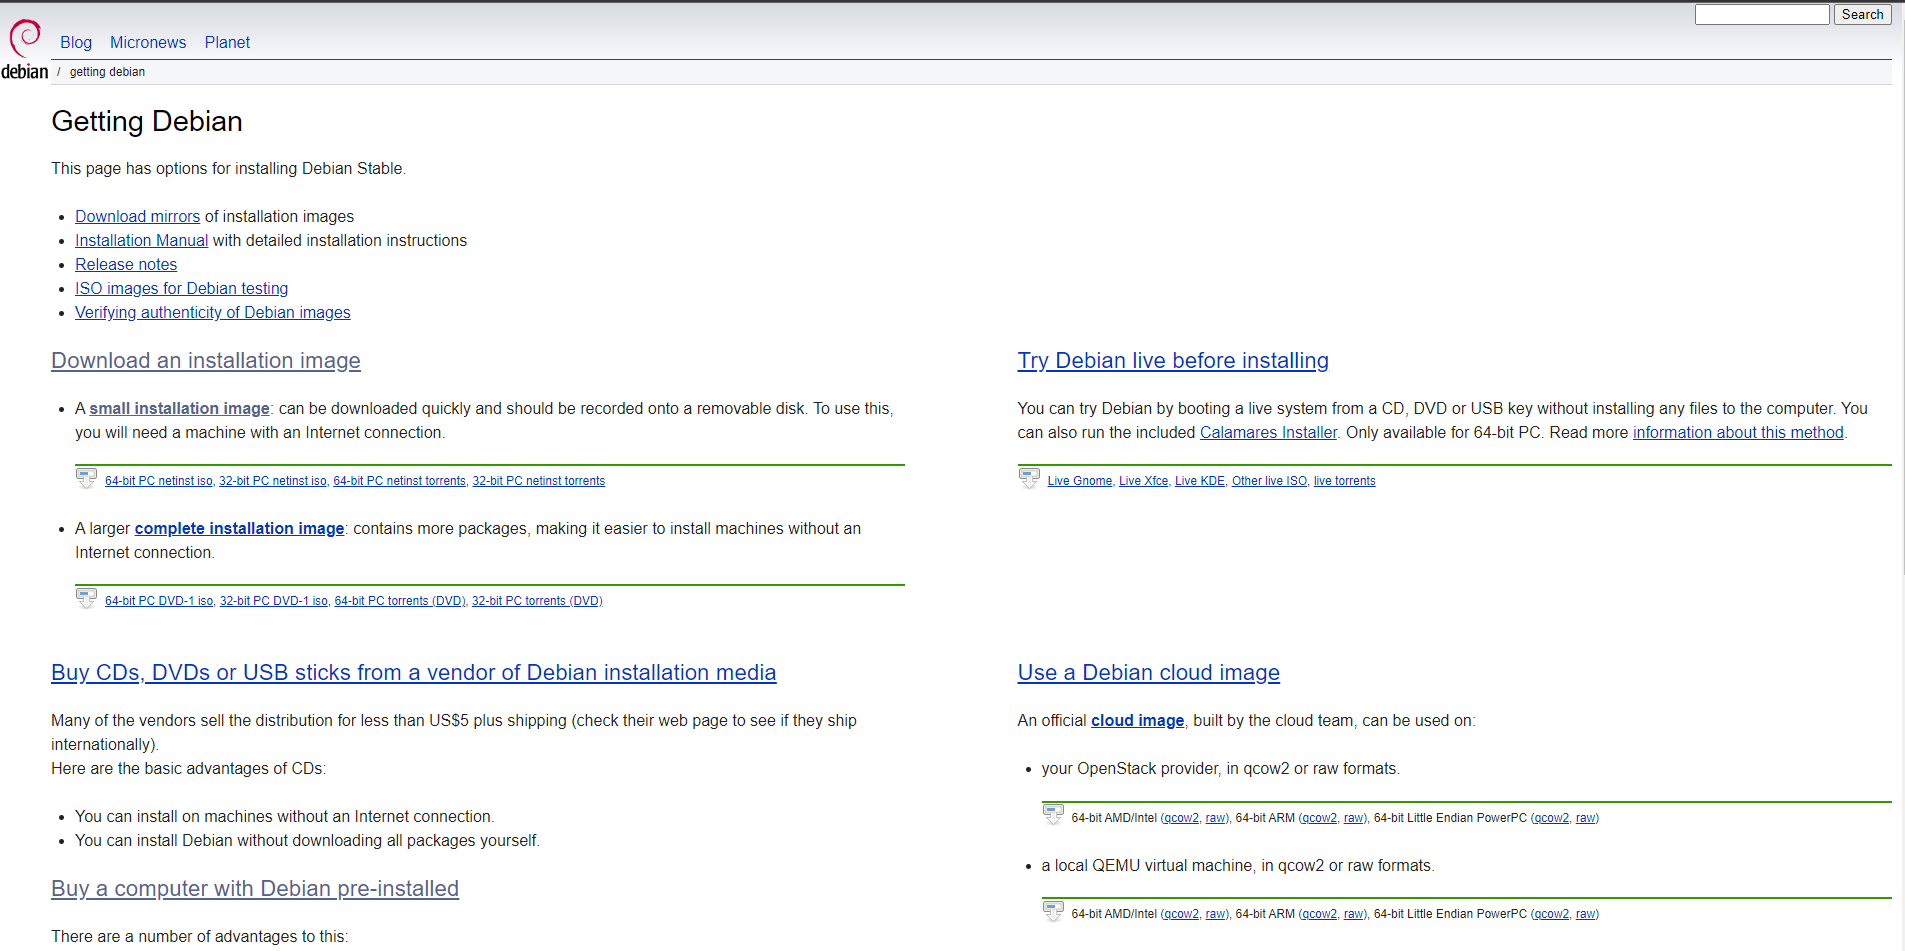
\includegraphics[width=0.5\linewidth]{instalacionBacula/debianPaginaWeb.png}
    \caption{Página de descarga de Debian}
\end{figure}

\textbf{Creación de la Máquina Virtual}\medskip


En VirtualBox, procedemos a añadir una nueva máquina virtual. Asignamos un nombre a la máquina y seleccionamos la imagen ISO de Debian descargada previamente.

\begin{figure}[H]
    \centering
    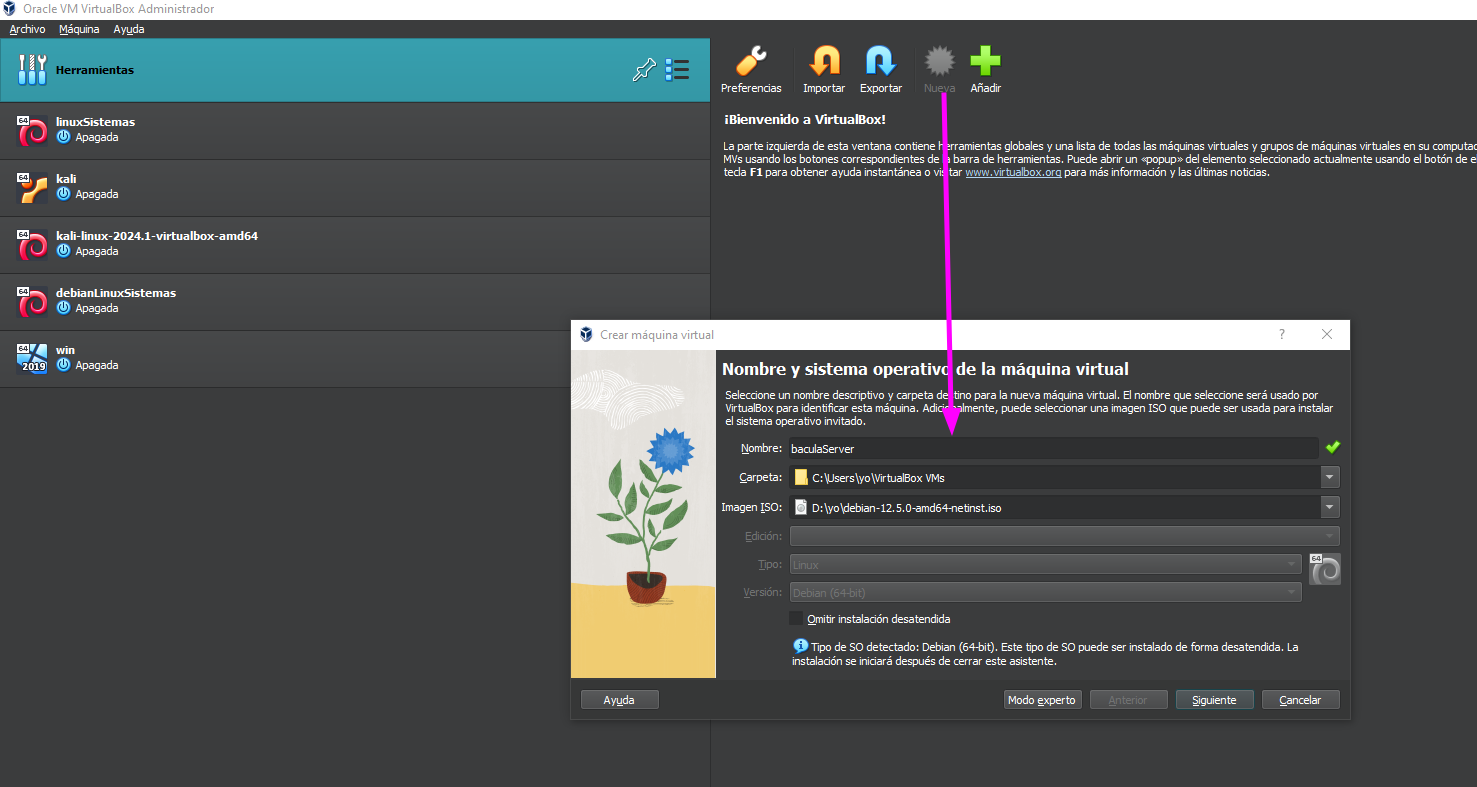
\includegraphics[width=0.5\linewidth]{instalacionBacula/vbDebian.png}
    \caption{Configuración inicial de la máquina virtual en VirtualBox}
\end{figure}

\textbf{Configuración del Usuario y Contraseña}\medskip


Configuramos el usuario y la contraseña que se utilizarán en la máquina virtual.

\begin{figure}[H]
    \centering
    \includegraphics[width=0.5\linewidth]{instalacionBacula/instalación desatendida del SO.png}
    \caption{Establecimiento de usuario y contraseña durante la instalación desatendida}
\end{figure}

\textbf{Configuración del Hardware}\medskip


Debian no requiere muchos recursos para operar de forma fluida. Por tanto, asignamos una cantidad moderada de memoria y procesadores.

\begin{figure}[H]
    \centering
    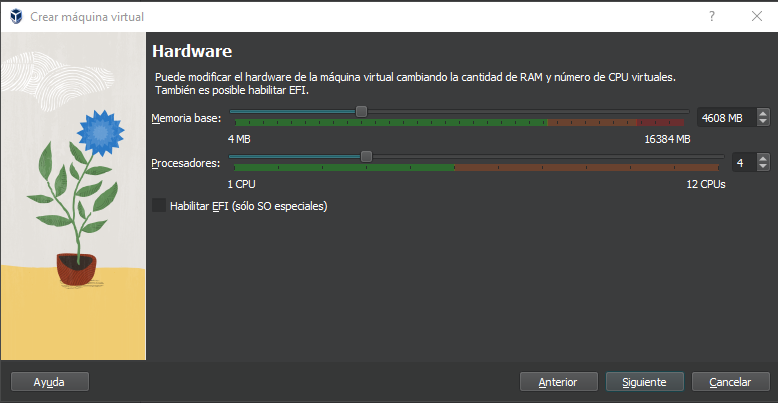
\includegraphics[width=0.5\linewidth]{instalacionBacula/vbhardware.png}
    \caption{Configuración del hardware en VirtualBox}
\end{figure}

\textbf{Asignación de Almacenamiento}\medskip


Creamos un disco duro virtual para la máquina y asignamos un espacio de 50 GB.

\begin{figure}[H]
    \centering
    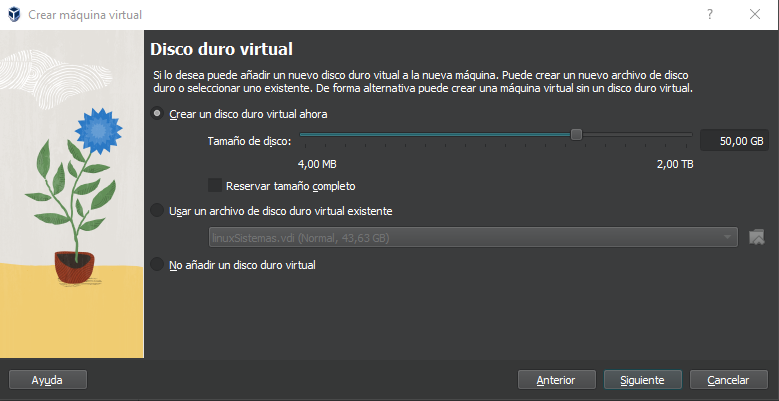
\includegraphics[width=0.5\linewidth]{instalacionBacula/vbDisco.png}
    \caption{Asignación de espacio en el disco duro virtual}
\end{figure}

\textbf{Instalación del Sistema Operativo}\medskip


Iniciamos la instalación de Debian y dejamos que el instalador complete el proceso.

\textbf{Actualización del Sistema}\medskip


Una vez instalado el sistema, ejecutamos comandos de actualización y mejora para asegurarnos de que tenemos la última versión de los paquetes.

\begin{figure}[H]
    \centering
    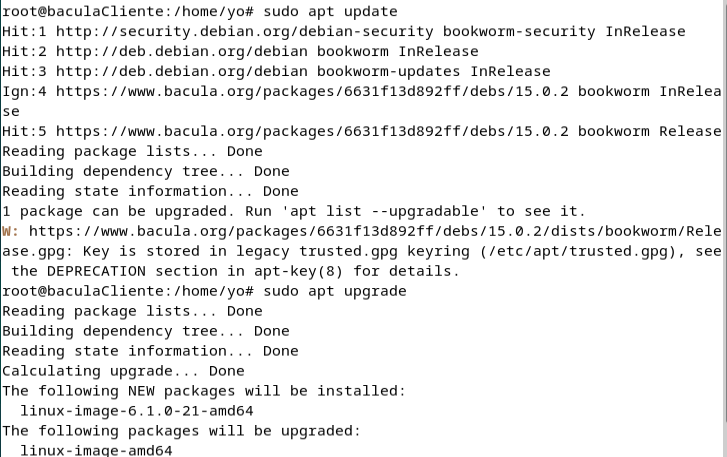
\includegraphics[width=0.5\linewidth]{instalacionBacula/Update y upgrade.png}
    \caption{Proceso de actualización y mejora del sistema}
\end{figure}

\textbf{Configuración de Red}\medskip


Finalmente, ajustamos la configuración de red de NAT a adaptador puente para facilitar la conectividad externa de la máquina virtual.

\begin{figure}[H]
    \centering
    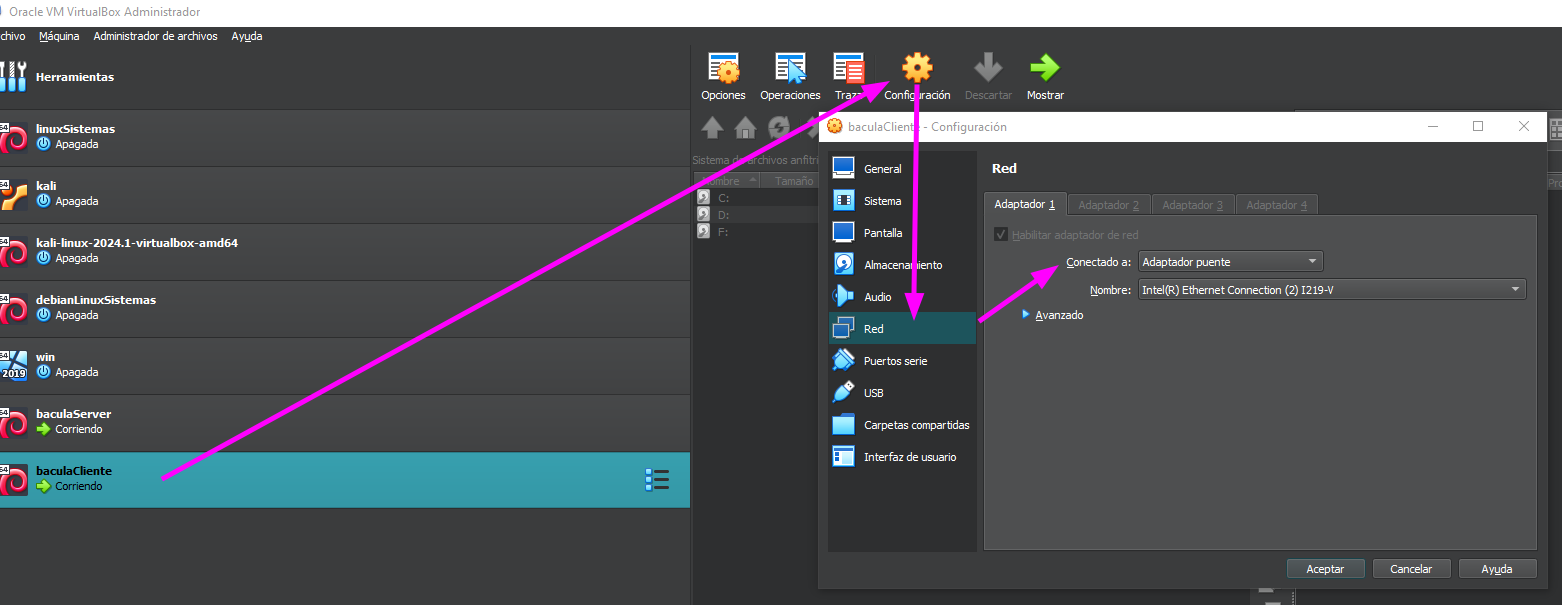
\includegraphics[width=0.5\linewidth]{instalacionBacula/NatAdaptadorPuente.png}
    \caption{Cambio de configuración de red a adaptador puente}
\end{figure}

